% Paper to publish our results from the IR SED fitting of the
% BAT AGN.
% Basic LaTex structure from MNRAS template on Overleaf
\documentclass[fleqn, usenatbib]{mnras}
\usepackage{newtxtext,newtxmath}
% Depending on your LaTeX fonts installation, you might get better results with one of these:
%\usepackage{mathptmx}
%\usepackage{txfonts}

\usepackage[T1]{fontenc}
\usepackage{ae,aecompl}


%%%%% AUTHORS - PLACE YOUR OWN PACKAGES HERE %%%%%

% Only include extra packages if you really need them. Common packages are:
\usepackage{graphicx}	% Including figure files
\usepackage{amsmath}	% Advanced maths commands
\usepackage{amssymb}	% Extra maths symbols
\usepackage{amsfonts}
\usepackage[flushleft]{threeparttable}
\usepackage{booktabs}
\usepackage{pdflscape}
\usepackage{caption}
%%%%%%%%%%%%%%%%%%%%%%%%%%%%%%%%%%%%%%%%%%%%%%%%%%

%%%%% AUTHORS - PLACE YOUR OWN COMMANDS HERE %%%%%

% Please keep new commands to a minimum, and use \newcommand not \def to avoid
% overwriting existing commands. Example:
%\newcommand{\pcm}{\,cm$^{-2}$}	% per cm-squared
\newcommand{\herschel}{\emph{Herschel}}
\newcommand{\swift}{\textit{Swift}}
\newcommand{\msun}{M$_{\sun}$}
\newcommand{\mstar}{$M_{\mathrm{star}}$}
\newcommand{\lsun}{L$_{\sun}$}
\newcommand{\mdust}{$M_{\rm dust}$}
\newcommand{\tdust}{$T_{\rm dust}$}
%%%%%%%%%%%%%%%%%%%%%%%%%%%%%%%%%%%%%%%%%%%%%%%%%%

%%%%%%%%%%%%%%%%%%% TITLE PAGE %%%%%%%%%%%%%%%%%%%

% Title of the paper, and the short title which is used in the headers.
% Keep the title short and informative.
\title[\emph{Herschel}-BAT Sample: AGN-SF Connection]{\emph{Herschel} far-infrared photometry of the Swift Burst Alert
Telescope active galactic nuclei sample of the local universe--III. The connection between nuclear activity and global star formation\thanks{{\it Herschel} is an ESA space observatory with science instruments provided by European-led Principal Investigator consortia and with important participation from NASA.}}

% The list of authors, and the short list which is used in the headers.
% If you need two or more lines of authors, add an extra line using \newauthor
\author[T. T. Shimizu]{T. Taro Shimizu$^{1}$\thanks{Email: tshimizu@astro.umd.edu}, Richard F. Mushotzky$^1$, Marcio Mel\'endez$^1$, Michael J. Koss$^{2}$, \newauthor Amy J. Barger$^{3,4,5}$, and Lennox L. Cowie$^{5}$\\
$^{1}$Department of Astronomy, University of Maryland, College Park, MD 20742, USA\\
$^{2}$Institute for Astronomy, Department of Physics, ETH Zurich, Wolfgang-Pauli-Strasse 27, CH-8093 Zurich, Switzerland\\
$^{3}$Department of Astronomy, University of Wisconsin-Madison, 475 N. Charter Street, Madison, WI 53706, USA\\
$^{4}$Department of Physics and Astronomy, University of Hawaii, 2505 Correa Road, Honolulu, HI 96822, USA\\
$^{5}$Institute for Astronomy, University of Hawaii, 2680 Woodlawn Drive, Honolulu, HI 96822, USA}

% These dates will be filled out by the publisher
\date{Accepted XXX. Received YYY; in original form ZZZ}

% Enter the current year, for the copyright statements etc.
\pubyear{2016}

% Don't change these lines
\begin{document}
\label{firstpage}
\pagerange{\pageref{firstpage}--\pageref{lastpage}}
\maketitle

% Abstract of the paper
\begin{abstract}

\end{abstract}

% Select between one and six entries from the list of approved keywords.
% Don't make up new ones.
\begin{keywords}
galaxies: active -- galaxies: Seyfert -- infrared: galaxies -- galaxies: star formation -- galaxies: evolution 
\end{keywords}

%%%%%%%%%%%%%%%%%%%%%%%%%%%%%%%%%%%%%%%%%%%%%%%%%%

%%%%%%%%%%%%%%%%% BODY OF PAPER %%%%%%%%%%%%%%%%%%

\section{Introduction}

\section{\herschel-BAT Sample}
Because \swift/BAT continuously monitors the entire sky in the energy range 14--195 keV for gamma ray bursts, it simultaneously provides an all-sky survey at ultra high X-ray energies. This allows for the creation of complete catalogs with increasing sensitivity the longer \swift/BAT remains in operations. Given the extreme environments necessary to produce strong 14--195 keV emission, the majority of sources in the \swift/BAT catalogues are AGN.

We chose 313 AGN from the parent sample of $\sim720$ AGN detected in the 58 month catalogue\footnote{\url{https://swift.gsfc.nasa.gov/results/bs58mon}} after imposing a redshift cutoff of $z<0.05$ and excluding Blazars and BL Lac objects to form our \herschel-BAT AGN sample. With a mean redshift of $\left<z\right> = 0.025$, our AGN sample provides a comprehensive view of the properties of AGN host galaxies in the local universe. Our selection at ultra high X-ray energies further removes biases and selection effects due to host galaxy contamination and obscuration \citep{Mushotzky:2004gf} that can influence samples at other wavelengths.   

The demographics of our sample are nearly evenly split between unabsorbed (Type I, 43 per cent) and absorbed AGN (Type II, 53 per cent) with the remaining 4 per cent (5 objects) either a Low-Ionization Nuclear Emission-line Region (LINER) or unclassified. For a complete listing of our sample with names, luminosity distances, redshifts, and AGN type, we point the reader to \citet{Melendez:2014yu} or \citet{Shimizu:2016qy}.

\section{Data}
\subsection{\herschel{} Photometry}
293 of the \herschel{}-BAT AGN were observed with \herschel{} \citep{Pilbratt:2010rz} as part of a Cycle 1 open time program (OT1\_rmushotz\_1, PI: Richard Mushotzky). The remaining 20 sources were part of the other programs with public archival data. \herschel{} observed all 313 AGN using both the Photoconductor Array Camera and Spectrometer \citep[PACS;][]{Poglitsch:2010fp} and Spectral and Photometric Imaging Receiver \citep[SPIRE;][]{Griffin:2010sf} producing images in five wavebands: 70, 160, 250, 350, and 500 \micron.

Detailed descriptions of the data reduction process and photometric flux extraction can be found in \citet{Melendez:2014yu} for PACS and \citet{Shimizu:2016qy} for SPIRE. The following is a short description of the flux extraction procedure. We measured fluxes at each waveband directly from the images using aperture photometry with a concentric annulus to define the local background. We applied aperture corrections for sources where we used a point source aperture as defined in the respective PACS and SPIRE data reduction guides. Fluxes for sources that were unresolved at all three wavebands in SPIRE were determined using the SPIRE Timeline Fitter within the \herschel{} Interactive Processing Environment. All fluxes have a signal-to-noise ratio of at least 5, otherwise we provided a 5$\sigma$ upper limit. 

\subsection{\textit{WISE} Photometry}
To extend the SEDs into the mid-infrared (MIR), we supplemented our \herschel{} data with archival \textit{Wide-field Infrared Survey Explorer} \citep[WISE;][]{Wright:2010fk} photometry. WISE performed a broadband all-sky survey at 3.4 (W1), 4.6 (W2), 12 (W3), and 22 (W3) \micron{} with angular resolution comparable to \herschel/PACS at 70 \micron{} for W1, W2, and W3 and 160 \micron{} for W4. We queried the AllWISE catalog through the NASA/IPAC Infrared Science Archive\footnote{\url{http://irsa.ipac.caltech.edu/frontpage/}} to search for coincident sources within 6". Counterparts were found for all but one AGN (Mrk 3) at every waveband. The catalog only contained W1 and W2 fluxes for Mrk 3 due to differences in the depth of coverage for W1/W2 and W3/W4.

The AllWISE catalog provides magnitudes determined using multiple extraction methods. We consider only the profile-fitting magnitudes (\textit{w}N\textit{mpro} where N is 1, 2, 3, or 4) and the elliptical aperture magnitudes (\textit{w}N\textit{gmag}). Profile-fitting magnitudes were determined by fitting the position dependent point spread function using deblending procedures when necessary to decompose overlapping sources. The \textit{w}N\textit{mpro} magnitudes therefore are only relevant for unresolved sources.

If a WISE source is associated with a source in the \textit{Two Micron All Sky Survey} (2MASS) Extended Source Catalog (XSC), then \textit{w}N\textit{gmag} magnitudes were also measured using an elliptical aperture with the same shape from the XSC and sizes scaled given the larger WISE beam. Thus, \textit{w}N\textit{gmag} magnitudes are more appropriate for extended sources. For details of all of the WISE magnitude measurements we point the reader to the All-Sky Release Explanatory Supplement\footnote{\url{http://wise2.ipac.caltech.edu/docs/release/allsky/expsup/}}.

Given the low-redshift nature of our sample, using only the \textit{w}N\textit{mpro} magnitudes would severely underestimate the flux for large extended sources. To decide which magnitude to include in the SED for each source, we used the reduced $\chi^{2}$ value (\textit{w}N\textit{rchi2}) from the profile-fitting. If \textit{w}N\textit{rchi2}$<3$ then we chose the \textit{w}N\textit{mpro} magnitude, otherwise \textit{w}N\textit{gmag} was chosen. 

\subsection{\emph{Spitzer}/IRS spectra}
To supplement the IR photometry, we searched the Cornell Atlas of Spitzer IRS Sources (CASSIS) (REFERENCE) for low-resolution Spitzer/IRS spectra. These MIR spectra span the 5-30 \micron{} wavelength range and can provide independent measures of the SFR and AGN fraction through the strength of emission features from different species such as polycyclic aromatic hydrocarbons (PAH), NeII, NeIII, and OIV. We can use the luminosity and equivalent width (EqW) of these features to test the reliability and accuracy of the properties from the broadband SED fitting. 

We can also test whether AGN heating has an effect on the dust composition of galaxies. Some studies (REFERENCES) have suggested that the hard ionizing radiation from the AGN has destroyed PAHs while others report no effect from the AGN. With our large sample covering a range of AGN luminosity and an independent measure of the SFR, we can definitively determine whether the AGN has an effect on the PAH abundance of galaxies.

We found 120/313 AGN on CASSIS and downloaded their reduced spectra using the default extraction method. Due to the different sizes of the Short-Low (SL) slit and Long-Low (LL) slit, the continuum of each can be offset mainly from extended emission not captured by the SL slit. Therefore spectral orders were stitched together by fitting a line to the ends of each order and scaling to match the overlapping regions. SL2 and LL2 were first matched and scaled to SL1 and LL1 respectively. Then the combined SL1/SL2 spectra was matched to the combined LL1/LL2 spectra to produce the final full Spitzer/IRS low resolution spectra. 

\section{Comparison Samples}
To test whether the AGN has any effect on the star-forming properties of their host galaxies, we need samples of galaxies which contain little evidence for nuclear activity. These samples also need to occupy the same redshift range to mitigate against evolutionary effects and have been observed with nearly the same instruments so the properties can be compared on an equal level. Therefore we chose to use the \herschel{} \textit{Reference Survey} \cite[HRS;][]{Boselli:2010fj} and the \textit{Key Insights on Nearby Galaxies: a Far-Infrared Survey with Herschel} \cite[KINGFISH;][]{Kennicutt:2011vn} galaxies as our comparison samples. In the following subsections we briefly describe these two surveys. For more detail, we direct the reader to the original survey publications.

\subsection{\herschel{} Reference Survey}
The HRS was a guaranteed time key \herschel{} program dedicated to studying the dust content of ``normal'' galaxies. The 323 galaxy sample is volume limited ($15< D < 25$ Mpc) to avoid distance effects and K-band flux limited to avoid selection effects due to dust and provide a representative population of local galaxies. The size of the HRS as well as the local nature make it an ideal sample to compare to the \herschel-BAT galaxies.

The HRS galaxies were imaged using both PACS and SPIRE, however the 100 \micron{} filter was used instead of the 70 \micron{} filter. \citet{Cortese:2014qq} and \citet{Ciesla:2012lq} measured the PACS and SPIRE flux densities respectively using similar techniques as the \herschel-BAT galaxies. WISE 12 and 22 \micron{} photometry for HRS were provided in \citet{Ciesla:2014qy}. The available data for the HRS SEDs are nearly identical as our sample. 

The only issue in comparing the HRS galaxies to the \herschel-BAT AGN concerns the stellar mass (\mstar) distribution. Because the near-infrared is most strongly effected by the mass of the older stellar population, the HRS K-band selection produces a \mstar{} distribution that is representative of the naturally occurring \mstar{} distribution. However, many recent studies have shown that AGN prefer high \mstar{} galaxies, a feature that is also found in the BAT AGN \citep{Koss:2011vn}. Figure~\ref{fig:mstar_dist} displays the \mstar{} distributions for the \herschel-BAT and comparison samples. The \herschel-BAT galaxies have an average \mstar{} of 10.6 \msun, whereas the average \mstar{} for HRS is 9.8 \msun, nearly a ten-fold difference. This will be important to account for in interpreting results from a comparison between the two samples.

\begin{figure}
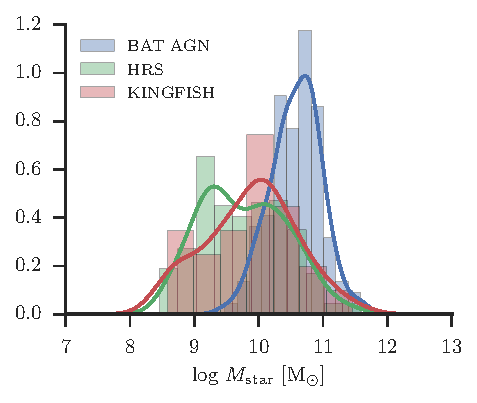
\includegraphics[width=\columnwidth]{figures/stellar_mass_comp}
\caption{Histograms and Kernel Density Estimates (KDE) of the \mstar{} distribution for the BAT AGN (blue), HRS (green), and KINGFISH (red) samples. The BAT AGN probe a higher \mstar{} galaxy population than non-AGN samples. A color version is available in the online publication. \label{fig:mstar_dist}}
\end{figure}

\subsection{KINGFISH Sample}
While the HRS galaxies were selected homogeneously, the KINGFISH galaxies are a heterogeneous sample selected to span the broad range of star-forming properties and ISM environments from dwarf galaxies to massive star-forming galaxies. Only 61 galaxies comprise the sample, 57 of which were part of the \textit{Spitzer} Infrared Nearby Galaxies Survey \citep[SINGS;][]{Kennicutt:2003wk}.

The KINGFISH galaxies were imaged at every \herschel{} waveband (70, 100, 160, 250, 350, and 500 \micron) using aperture photometry with flux densities provided by \citet{Dale:2012dq}. To cover the MIR portion of the SED, we used the \textit{Spitzer}/IRAC and MIPS 8 and 24 \micron{} data from \citet{Dale:2007fk}. Because the MIR data is from the SINGS survey, this reduces the KINGFISH sample from 61 to 57 galaxies. 

Various miscellaneous properties about each KINGFISH galaxy, including \mstar, were compiled from \citet{Kennicutt:2011vn}. We removed all galaxies with $\log($\mstar$)<8.0$ \msun{} because all are dwarf galaxies that are not represented in the \herschel-BAT sample. The final \mstar{} distribution for the KINGFISH comparison sample is shown in Figure~\ref{fig:mstar_dist}. While the KINGFISH galaxies are located at slightly higher masses (mean $\log($\mstar$)=9.9$ \msun), the \herschel-BAT sample is still biased significantly towards higher stellar masses. 

An advantage of the KINGFISH sample is the availability of \textit{Spitzer}/IRS low-resolution spectra which were analyzed by \citet{Smith:2007lr}. The MIR emission feature measurements will be important for comparing their fluxes and luminosities to the FIR SED measured properties and assessing the effect of the AGN. 

\section{SED Model Fitting}
Many models and templates exist in the literature to fit the broadband SEDs of galaxies. In this work we particularly focus on four methods that range from analytic representations to empirical templates based on previous studies. The \herschel-BAT sample can uniquely test the viability of the various methods, particularly in the presence of an AGN. 

\subsection{Single modified blackbody}
One of the most widely used models for fitting the FIR SED of galaxies is a single modified blackbody (MBB). The simple model consists of a normal, single temperature blackbody that represents isotropic dust emission combined with a frequency dependent opacity given that dust is not a perfect blackbody.In the optically thin limit, the opacity can be approximated as a powerlaw, $\tau_{\nu}=(\nu/\nu_{0})^{\beta}$. The form of the single modified blackbody for the flux density at each frequency is then

\begin{equation}
S(\nu) \propto \nu^{\beta}B_{\nu}(T_{\mathrm{d}})
\end{equation}

\noindent where $\beta$ is the spectral emissivity index and $B_{\nu}(T_{\mathrm{d}})$ is the standard Planck blackbody function for an object with temperature $T_{\mathrm{d}}$. This simple model has been shown to fit well the prominent FIR bumps for large samples of star-forming galaxies [REFERENCES] and provides estimates of the dust temperature, dust mass, and SFR.

To calculate the dust mass, we must assume a particular dust absorption coefficient, $\kappa_{0}$ at a particular frequency, $\nu_{0}$. For this work, we assume $\kappa_{0}=0.192\,\mathrm{m^{2}\,kg^{-1}}$ and $\nu_{0}=857\,\mathrm{GHz}$ (i.e. 350 \micron) from \citet{Draine:2003gd}. However, as \citet{Bianchi:2013jk} shows, by assuming a specific $\kappa_{0}$, we must also fix the spectral emissivity index to the value used to measure $\kappa_{0}$. In this work, we fix $\beta=2.0$ to match spectral emissivity index used by \citet{Draine:2003gd}. The final full form of the single MBB model is then

\begin{equation}\label{eq:greybody}
S_{\mathrm{MBB}}(\nu) = \frac{M_{\mathrm{d}}\kappa_{0}}{D_{\mathrm{L}}^2}\left(\frac{\nu}{\nu_{0}}\right)^{\beta}\frac{2h\nu^{3}}{c^{2}}\frac{1}{e^{{h\nu/kT_{\mathrm{d}}}}-1}
\end{equation}

\noindent where $M_{\mathrm{d}}$ is the dust mass, $D_{\mathrm{L}}$ is the luminosity distance, $c$ is the speed of light, $h$ is the Planck constant, and $k$ is the Boltzmann constant. The two free parameters then are $M_{\mathrm{d}}$ and $T_{\mathrm{d}}$, the dust mass and dust temperature respectively.

\subsection{Casey 2012 model}
The simple assumption that dust emission in the IR can be modeled with a single temperature blackbody works well for ``normal'' star-forming galaxies. However for galaxies with large amounts of hot dust either due to a compact starburst or central AGN, this assumption can quickly break down. To account for this hot dust we also fit our sample using the model described in \citet[][hereafter C12]{Casey:2012jl} which is the combination of a single MBB and an exponentially cutoff powerlaw. The C12 model takes the form

\begin{equation}\label{eq:casey}
S_{\mathrm{C12}}(\nu) = N_{\mathrm{pl}}\left(\frac{\nu}{\nu_{\mathrm{c}}}\right)^{-\alpha}e^{-\nu_{\mathrm{c}}/\nu}S_{\mathrm{MBB}}(\nu)
\end{equation}

\noindent where $\nu_{\mathrm{c}}$ represents the turnover frequency and $N_{\mathrm{PL}}$ is a normalization constant. C12 illustrated using the \textit{Great Origins All-Sky LIRG Survey} (GOALS) sample that this model provides better estimates of the cold dust temperature, dust mass, and IR luminosity compared to both a single temperature modified blackbody and template libraries.

The C12 model introduces three more free parameters ($N_{\mathrm{PL}}$, $\alpha$, and $\nu_{\mathrm{c}}$) however within the implementation used by C12, $N_{\mathrm{PL}}$ and $\nu_{\mathrm{c}}$ are tied to the normalization of the modified blackbody component and dust temperature to produce a smoothly varying SED and reduce the number of free parameters from five to three. 

However, after early tests using this initial setup, we found that fixing $N_{\mathrm{PL}}$ and $\nu_{\mathrm{c}}$ as a function of the other parameters produced unreliable fits. This is because AGN SEDs from the MIR to FIR are not as smooth as those seen in (U)LIRGS, likely due to the disconnect between star-formation and AGN heating. Within starbursting galaxies both the hot and cold dust are related through the same heating process, i.e. star formation, while the much of the MIR emission in AGN host galaxies originates from dust around the AGN with no strong connection to global star formation in the galaxy. Therefore, we chose to leave both $N_{\mathrm{PL}}$ and $\nu_{\mathrm{c}}$ as free parameters resulting in a total of five for the entire model.

\subsection{DecompIR model}
Besides analytic models, another popular method is the use of template SEDs. Templates are constructed based on well-sampled SEDs of large samples of galaxies and usually parameterized according to a known property such as infrared luminosity.

For galaxies known to host an AGN, recent studies have turned to the \textsc{DecompIR} \citep{Mullaney:2011yq} templates. \textsc{DecompIR} consists of five host galaxy templates that span the IR color and luminosity range of the original \citet{Brandl:2006kx} starburst galaxy templates. \citet{Mullaney:2011yq} constructed the AGN templates based on a subsample of the \swift/BAT AGN which had AGN dominated \textit{Spitzer}/IRS spectra determined by the EqW of the 11.3 \micron{} feature being $<0.03$ \micron. The \textit{Spitzer}/IRS spectra were combined with \textit{IRAS} photometry at 60 and 100 \micron to define the ``intrinsic'' AGN SED from 6--100 \micron. 

\citet{Mullaney:2011yq} created three different AGN templates: one based only on high AGN luminosity objects, low AGN luminosity objects, and a median of the entire sample. For this work, we only consider the median AGN template given our SEDs only contain two points in the MIR where AGN-related emission is expected to dominate. 

\subsection{Dale et al 2014 model}
The third model we chose to test on our sample is the semi-empirical templates from \citet[][hereafter D14]{Dale:2014yq}. These templates also contain two components, one for dust emission in the host galaxy and one for the AGN. The host galaxy components were built from an updated version of the \citet{Dale:2002ty} model. Each component represents an SED produced using a different value of $\alpha_{\mathrm SF}$, which is the powerlaw slope of the intensity distribution for the interstellar radiation field that is heating the dust. These SEDs contain a mixture of emission from PAHs, small stochastically heated grains, and thermally radiating large grains.

For the AGN component, D14 chose the median SED of the Palomar-Green quasars from \citet{Shi:2013vn} citing the care with which any star-forming component was removed and the prominence of several AGN related MIR features such as the [OIV] fine structure line and the broad 10 and 18 \micron{} silicate emission bumps. At long wavelengths the AGN template falls as a blackbody.

Instead of two separate templates for the AGN and host galaxy, D14 provided a single set of templates based on different combinations of $\alpha_{\mathrm SF}$ and $f_{\mathrm AGN}$, the fractional contribution of the AGN to the 5--20 \micron{} emission. In total there are 1365 templates that range in $\alpha_{\mathrm SF}=0.0625-4.0$ in 0.0625 intervals and $f_{\mathrm AGN} = 0-1$ in 0.05 intervals.

\subsection{SED Fitting Methods}
We used two different fitting methods to fit the SEDs of the galaxies: 1) a Bayesian framework including Monte Carlo Markov Chain (MCMC) analysis for parameter estimation and 2) maximum likelihood optimization. For the analytic models (single modified blackbody and C12), we chose the Bayesian framework, and for the template based models (DecompIR and D14) we chose maximum likelihood optimization. The main reason for using two different methods to determine the best fit model SED is that the Bayesian framework does not work well with a set of discrete model templates, especially when the number of templates is low. Further, the only parameter in the template fitting that needs to be optimized is the normalization of the template to fit the observed SED. With a uniform prior on the one parameter, Bayesian methods essentially are reduced to maximum likelihood optimization.

\subsubsection{Maximum Likelihood Optimization}
We begin the maximum likelihood method because the main component underlying both methods is the definition of the likelihood. The likelihood defines the probability of a set of data given a specific model. In SED fitting, this translates to the combined probability of measuring all the photometric data points in the observed SED given a model for the SED (whether based on templates or analytic models). The total likelihood can then be expressed as the product of the probabilities of observing each single photometric point:

\begin{equation}\label{eq:likelihood}
\mathcal{L}(F|M) = \prod_{i}P(F_i|M)
\end{equation}

\noindent where $F$ is the set of photometric fluxes, $F_i$ and $M$ is the model. For our analysis, we assume the probability of our observations follow a Gaussian distribution with mean equal to $M$ and standard deviations equal to the measurement errors, $\sigma_{i}$.

\begin{equation}\label{eq:detected_prob}
P(F_i|M) = \frac{1}{\sqrt{2\pi\sigma_{i}^{2}}}\mathrm{exp}\left(\frac{-(F_i - M)^2}{2\sigma_i^2}\right)
\end{equation}

Equation~\ref{eq:detected_prob} only defines the probability for detected fluxes. To use the information contained in the undetected photometry, $U_i$, we define a different probability under the assumption that all of the upper limits are 5$\sigma$. 

\begin{align}\label{eq:undetected_prob}
P(U_i|M) &= \int_{-\infty}^{U_i}\frac{1}{\sqrt{2\pi\sigma_{i}^{2}}}\mathrm{exp}\left(\frac{-(x - M)^2}{2\sigma_i^2}\right)dx \notag\\
&= \frac{1}{2}\left(1 + \mathrm{erf}\left[\frac{U_i - M}{\sigma_i\sqrt{2}}\right]\right) 
\end{align}

\noindent where $\sigma_i = \frac{U_i}{5}$ and erf is the standard error function. For numerical accuracy and simplicity, it is customary to minimize the negative log-likelihood. Supposing we have $N$ total SED points with $D$ detections and $D-N$ non-detections then the total negative log-likelihood combining Equations~\ref{eq:likelihood},~\ref{eq:detected_prob},~and~\ref{eq:undetected_prob} is:

\begin{align}\label{eq:log_like}
-\log\mathcal{L} = \frac{1}{2}&\sum_{i=0}^{D}\left[\log(2\pi\sigma_i^2) - \left(\frac{F_i - M}{\sigma_i}\right)^2\right] + \notag \\
&\sum_{j=0}^{D-N}\log\left[1 + \mathrm{erf}\left(\frac{U_j - M}{\sigma_j\sqrt{2}}\right)\right]
\end{align}

It is important to recognize here how $M$ is calculated, no matter whether it represents a template or analytic model. Each data point in an SED is the observer-frame flux density measured over a defined wavelength range. Therefore, to determine the model flux densities we first redshifted the full rest-frame model SED into the observer frame using the known redshifts of all of our sources. This observer-frame SED was then convolved with each instrument filter transmission curve to produce model flux densities that can be accurately compared to the observed ones.

For each template in a model set, Equation~\ref{eq:log_like} was minimized to determine the best fit normalization. We then chose the normalized template with the lowest $-\log\mathcal{L}$ as the best fitting model for a source. For the DecompIR set, this meant first simultaneously optimizing over a normalization for the AGN component and each host galaxy component, then choosing the combined template that resulted in the minimum $-\log\mathcal{L}$. For D14, this meant calculating $-\log\mathcal{L}$ over the entire set of $\alpha$ and $f_{AGN}$ templates.

Uncertainties using the maximum likelihood method were determined by generating 1000 simulated SEDs for each source. These data points in the simulated SEDs were calculated by assuming each detected point followed a Gaussian distribution with mean equal to the observed flux density and a standard deviation equal to the measured error. Each of the simulated SEDs were re-fit using the same method. The standard deviation on the set of best fit parameters from the simulated SEDs then was used as the uncertainty. In this way both statistical and systematic errors can be taken into account in assessing the reliability of our best fit parameters. 

\subsubsection{Bayesian MCMC Analysis}
Within the Bayesian framework, the important probability is the probability of the model given the data at hand, i.e. the most probable SED model given the observed fluxes. This probability can be determined using Bayes theorem:

\begin{equation}\label{eq:bayes}
P(M|F) = \frac{P(F|M)P(M)}{P(F)}
\end{equation}

\noindent and is known as the posterior probability distribution. $P(F|M)$ is proportional to the likelihood (Equation~\ref{eq:likelihood}), $P(M)$ codifies our prior knowledge about the model, and $P(F)$ is the model evidence and can be disregarded as a simple normalization term. 

The reader may notice that assuming a flat prior, $P(M) \propto 1$, reduces Equation~\ref{eq:bayes} to $P(M|F) \propto \mathcal{L}$ verifying our use of maximum likelihood in determining the best template models.

For the single MBB and C12 models, we used flat priors for the dust temperature and dust mass. We placed conservative limits on both the dust temperature and $\log M_{\mathrm dust}$ to be between 1 and 100 K and 1 and 10 \msun respectively. Within the powerlaw component for the C12 model, we also used flat priors for the powerlaw slope between -5 and 5 and the log of the normalization between -10 and 10. Based on previous work attempting to measure the intrinsic AGN SED and modeling the dusty torus, we expect the SED to turnover anywhere in the range between 20-70 \micron. Therefore we imposed a Gaussian prior centered at 45 \micron{} with a standard deviation of 20 \micron. We found that imposing this prior resulted in better and more realistic fits to the SEDs.

We used the \textsc{PYTHON} package \textsc{emcee} \citep{Foreman-Mackey:2013lr} to perform MCMC and sample the posterior probability distribution function (Equation~\ref{eq:bayes}). \textsc{emcee} runs an implementation of the Affine-Invariant MCMC sampler from Goodman \& Weare 2010. Instead of one single MCMC chain, it samples the posterior PDF with multiple ``walkers'', each with their own chain. For our analysis, we used 50 walkers that each produced a 1000 step chain. To allow for each chain to stabilize and move away from the initial guesses for the parameters, we imposed a 200 step ``burn-in''. In total, this resulted in 40000 steps to define the full posterior PDF. 

To determine the best fit parameters, we first marginalized the posterior PDF over all other parameters and then calculated the median. All quoted uncertainties represent the 68\% confidence interval determined from the 16th and 84th percentile of the marginalized posterior PDF.

For sources with less than four detections in their SED, we fixed the dust temperature to 25 K since the peak of the FIR bump is no longer constrained. In these cases, we only obtained upper limits on the dust mass by calculating the upper 95th percentile of the marginalized PDF.

\section{Results}
We fit the \herschel-BAT sample using all three models. Best fit parameters for the C12, DecompIR, and D14 models are provided in Tables~\ref{tab:c12_params}, \ref{tab:decompir_params}, and \ref{tab:d14_params}. We also fit the HRS and KINGFISH samples using the C12 model to compare the dust and star-forming properties of non-AGN and AGN host galaxies. 

\subsection{Luminosities and AGN Fractions}
In addition to the parameters associated for each model, we also calculated luminosities and AGN fractions. For the this work, we define three luminosities: 1) $L_{\rm IR}$ will represent the total infrared luminosity determined by integrating the SED from 8--1000 \micron. 2) $L_{\rm SF}$ will represent the 8--1000 \micron{} luminosity due to star formation in the host galaxy. 3) $L_{\rm AGN, IR}$ will represent the 8--1000 \micron luminosity due to the AGN-heated dust. 

For the DecompIR template set, $L_{\rm IR}$, $L_{\rm SF}$, and $L_{\rm AGN, IR}$ were simply calculated from the best fit total, host galaxy, and AGN SEDs. For the D14 model set, $L_{\rm IR}$ was measured from the best fitting template and $L_{\rm SF}$ and $L_{\rm AGN, IR}$ were calculated based on the best fit $f_{\rm AGN}$.\footnote{\citet{Dale:2014yq} only provides $f_{\rm AGN}$ calculated between 5--15 \micron, however D. Dale graciously provided the authors with $f_{\rm AGN}$ calculated between 8--1000 \micron{} through private communication in August 2015.} Uncertainties on all of these luminosities were determined using the same Monte Carlo method used to determine the uncertainties on the best fitting parameters.

For the C12 model, we also measured $L_{\rm IR}$ by integrating the best fit total SED from 8--1000 \micron. However, we have decomposed the SED into two components: the powerlaw (PL) and MBB component. Naively, if we assumed the MIR powerlaw component is completely dominated by the AGN for all sources then we could just take the ratio as we did for the template models. This is not the case though as some sources have much of their MIR emission originating in the host galaxy. Therefore we must correct for host galaxy MIR emission associated with star formation.

We make this correction using the results of the C12 modeling for the HRS and KINGFISH samples. Since all of the galaxies in these samples have either no or low-luminosity AGN, the MIR emission is primarily the result of stochastically heated grains near star-forming regions and highly likely not associated with an AGN. In Figure~\ref{fig:lmbb_lpl_ratio}, we show the distribution of $L_{\rm MBB}/L_{\rm PL}$, the ratio of the MBB component luminosity to the MIR powerlaw component. The ratios for the HRS and KINGFISH samples are both narrowly distributed around a single value, indicating that for non-AGN galaxies the energy contained in the PL and MBB components are tightly connected. Combining both the HRS and KINGFISH samples, we find a median $\log(L_{\rm MBB}/L_{\rm PL})=0.48 \pm 0.11$, which transforms to $L_{\rm PL,SF} \approx \frac{1}{3}L_{\rm MBB}$ where we now indicate the contribution to the PL component from star formation as  $L_{\rm PL,SF}$. We can calculate the AGN contribution for the BAT AGN then by assuming the star-forming emission follows the same ratio.

\begin{align}
L_{\rm AGN,\,IR} &= L_{\rm PL} - L_{\rm PL, SF} = L_{\rm PL} - \frac{1}{3}L_{\rm MBB} \label{eq:c12_lagnIR} \\
f_{\rm AGN, C12} &= L_{\rm AGN, \, IR}/L_{\rm IR} \label{eq:c12_fagn} \\
L_{\rm SF, C12} &= L_{\rm MBB} + L_{\rm PL,SF} =  \frac{4}{3}L_{\rm MBB} \label{eq:c12_lsf}
\end{align}

By using these relatively simple corrections we can accurately compare luminosities and AGN fractions from the three different models.
\begin{figure}
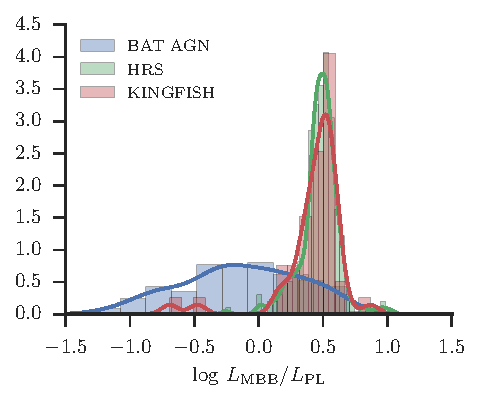
\includegraphics[width=\columnwidth]{figures/lmbb-lpl-ratio}
\caption{Histograms and Kernel Density Estimates (KDE) of the $L_{\rm MBB}/L_{\rm PL}$, distribution for the BAT AGN (blue), HRS (green), and KINGFISH (red) samples. The non-AGN samples have a narrowly distributed ratio whereas the BAT AGN span a wide range due to the AGN contribution. A color version of this figure is available in the online publication. \label{fig:lmbb_lpl_ratio}}
\end{figure}

\subsection{Comparison between models}
The measured property that should be most model independent is the total infrared luminosity, $L_{\rm IR}$. Assuming each model was able to fit well the broadband SEDs and reproduce the observed photometry, $L_{\rm IR}$ is simply the total integrated energy underneath the SED, irregardless of how the SED is decomposed. In Figure~\ref{fig:lir_total_comp}, we plot the correlations between each of the $L_{\rm IR}$ in the off-diagonal subplots as well as the single distributions for each one. 

The median $\log\,L_{\rm IR}$ for the C12, DecompIR, and D14 models are 10.43, 10.44, and 10.63 \lsun respectively and each model showing a spread of 0.5 dex. Based on the medians as well as Figure~\ref{fig:lir_total_comp}, the C12 and DecompIR models best agree. The average logarithmic difference between them is only -0.02 dex while the average difference between the D14 and C12 and DecompIR models is 0.2 dex, indicating a factor of 1.6 increase in $L_{\rm IR}$ between D14 and the other two models. This is due to the shape of the template SEDs for D14. D14's AGN template is flatter at shorter wavelengths causing the increased luminosity. 

The strict set of templates available in the D14 model also likely causes the increased scatter between D14 and the two others. Whereas DecompIR is composed of two templates that can freely float to match the observed SED and the C12 model is analytical allowing for large flexibility, the D14 model just contains a fixed set of templates which might not be able to match the observed SED as well as the other two models.

Despite these differences, overall there is great agreement, as expected, between the measurement of $L_{\rm IR}$ for the three models. Given the 0.2 dex difference between D14 and the C12 and DecompIR models, we can conservatively assign this value as the total uncertainty on all $L_{\rm IR}$. This uncertainty overwhelms the individual statistical uncertainties which are $\sim0.03$ dex.

%%%%%%%%%%%%%%%%%%%%%%%% FIGURE: LIR COMPARISON %%%%%%%%%%%
\begin{figure*}
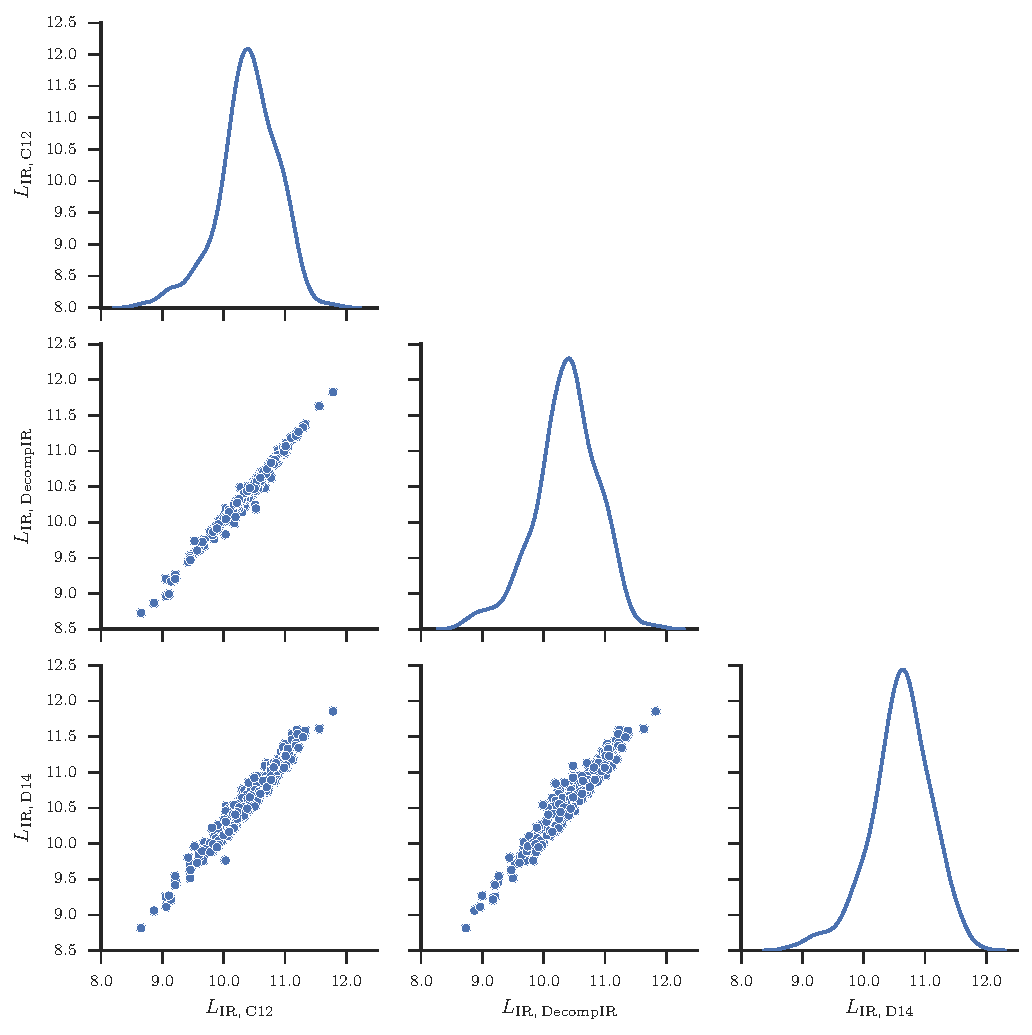
\includegraphics[width=\textwidth]{figures/lir_total-comparison}
\caption{Correlations and KDEs of $L_{\rm IR}$ from the three SED models.  A color version of this figure is available in the online publication. \label{fig:lir_total_comp}}
\end{figure*}
%%%%%%%%%%%%%%%%%%%%%%%%%%%%%%%%%%%%%%%%%%%%%%%%%%

Where the models begin to disagree more, is in the actual decomposition of the SED. In particular, we compare $f_{\rm AGN}$, the fraction of the 8--1000 \micron{} luminosity due to AGN-heated dust. In the previous section we outlined how this value was calculated for each model. For the template-based models (DecompIR and D14), this was simply the ratio of the luminosity from the AGN component template to the $L_{\rm IR}$ while for the C12 model, we needed to make a correction to account for MIR emission due to the host galaxy. 

Figure~\ref{fig:agn_frac_comp} displays the relationship between each model's $f_{\rm AGN}$ in the off-diagonal plots as well as the distribution of $f_{\rm AGN}$ in the diagonal plots. All three models are in rough agreement of $f_{\rm AGN}$. The three off-diagonal plots show a strong correlation between the models, albeit with large scatter. We find Pearson correlation coefficients of 0.81, 0.83, and 0.92 for C12 vs. DecompIR, C12 vs. D14, and DecompIR vs. D14 respectively. The two template based models agree the best between each other. This is likely due to the fixed shape of the AGN component SED for these models and the correction factor we had to use to calculate the C12 based $f_{\rm AGN}$. 

Overall all three models agree on $f_{\rm AGN}$ within a scatter of 0.15. The scatter around a 1--1 correlation (shown by the dashed black line) between each model is 0.15, 0.13, and 0.10 for C12 vs. DecompIR, C12 vs. D14, and DecompIR vs. D14 respectively. Because this is comparable to the statistical uncertainty we determined through the individual model-fitting, we add this in quadrature to the uncertainties in Tables~\ref{tab:c12_params},~\ref{tab:decompir_params},~and~\ref{tab:d14_params}. Interestingly in terms of following a 1--1 correlation, C12 and DecompIR compare the best even though between these two models the scatter is largest. We suspect this is due to the broad agreement in the shape of the AGN SED where both models have the AGN rising as a powerlaw with a slope $\sim2$ and peaking around 40 \micron{}. The D14 model has a flatter MIR slope that peaks closer to 20 \micron leading to the systematic offset seen in Figure~\ref{fig:agn_frac_comp}. The offset between D14 and the other two models is $\sim$0.1. 

The 15 per cent uncertainty between the three models represents our general lack of knowledge about the details of decomposing broadband SEDs of AGN host galaxies. The estimated $f_{\rm AGN}$ is highly dependent on the assumed models of both the host galaxy and AGN, and currently at best we can only constrain to within 15 per cent. This influences then the calculations of both the SFR (based on $L_{\rm SF}$) and the IR portion of AGN luminosity ($L_{\rm AGN, IR}$). Studies relying on calculating the SFR of AGN host galaxies using the infrared need to take these discrepancies into account or else risk over-interpreting results based on broad SED decomposition.

For our AGN population, we find almost a uniform distribution of $f_{\rm AGN}$ independent of the model used. Most AGN have between 20 and 80 per cent of their IR emission coming from AGN heated dust. This means that the IR SED of an AGN host galaxy can wildly vary from being completely dominated by star formation related emission to being completely dominated by AGN related emission. The next question then becomes: Which process is changing from AGN to AGN? Is star formation or AGN activity the main driver behind the differing $f_{\rm AGN}$ or perhaps a connection between the two causing one to decrease while the other increases? We explore this issue in a later section.

%%%%%%%%%%%%%%%%%%%%%%%% FIGURE: AGN FRACTION COMPARISON %%%%%%%%%%%
\begin{figure*}
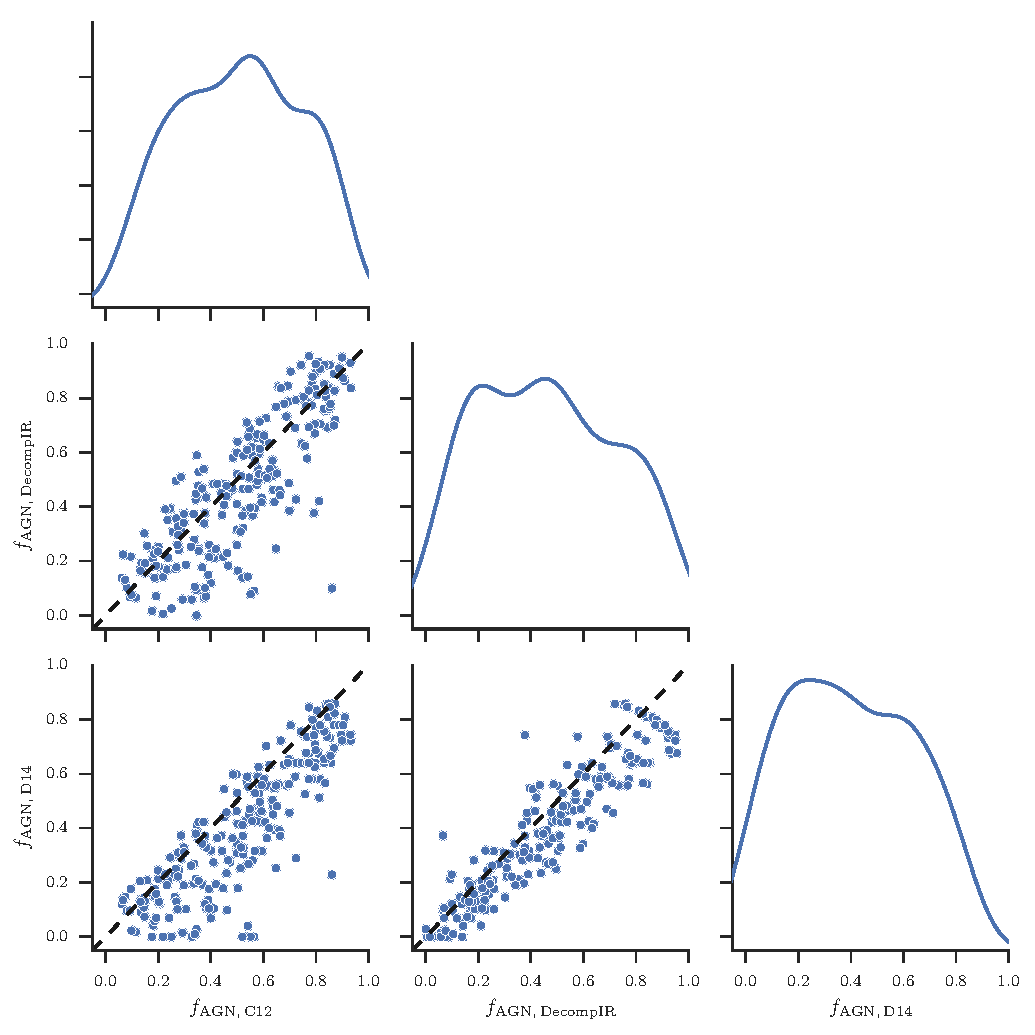
\includegraphics{figures/agn_frac-comparison}
\caption{Correlations and KDEs of $f_{\rm AGN}$ from the three SED models.  A color version of this figure is available in the online publication. \label{fig:agn_frac_comp}}
\end{figure*}
%%%%%%%%%%%%%%%%%%%%%%%%%%%%%%%%%%%%%%%%%%%%%%%%%%

\subsection{$M_{\rm dust}$, $T_{\rm dust}$, and SFR of local AGN host galaxies}
Given the results of the previous section, for the rest of the paper we will focus on properties determined using the C12 model since the model provides a wealth of information regarding not just the SFR but also the dust mass ($M_{\rm dust}$), dust temperature ($T_{\rm dust}$), MIR powerlaw slope, and turnover wavelength. We note that any results pertaining to the infrared luminosity of either the AGN or the host galaxy are broadly repeated using either of the other two models with only small changes in the statistics.

%%%%%%%%%%%%%%%%%%%%%%%% FIGURE: Mdust, Tdust, SFR COMPARISON %%%%%%%%%%%
\begin{figure*}
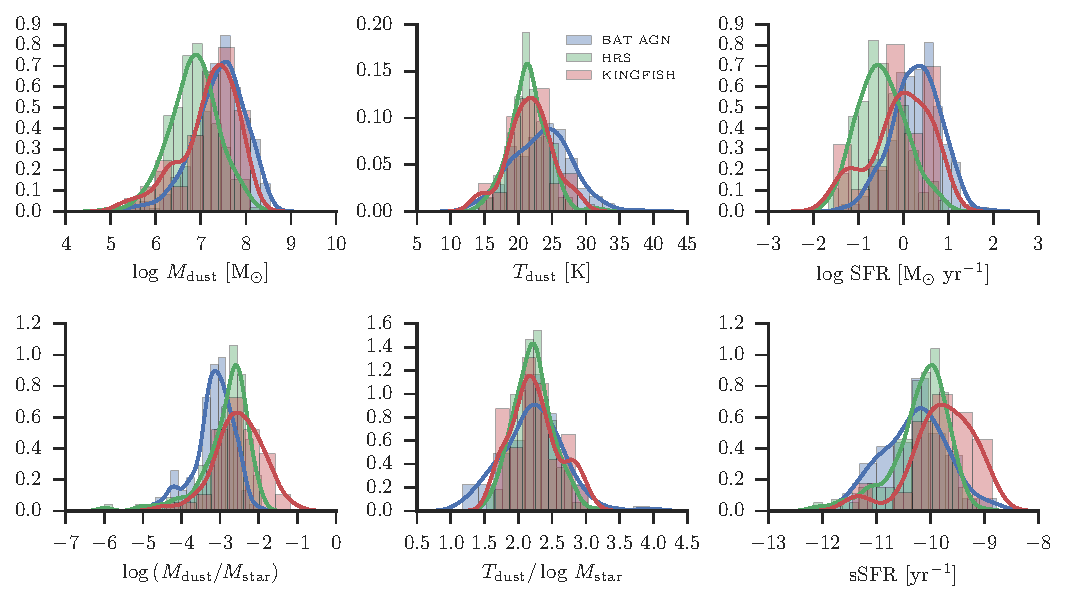
\includegraphics[width=\textwidth]{figures/mdust_tdust_sfr_comparison}
\caption{ Comparison of $M_{\rm dust}$, $T_{\rm dust}$, and SFR between the \herschel-BAT AGN (blue), HRS (green), and KINGFISH (red) samples. The top row compares the absolute values of these properties while the bottom row compares the properties normalized by $M_{\rm star}$. A color version of this figure is available in the online publication. \label{fig:mdust_tdust_sfr_comp}}
\end{figure*}
%%%%%%%%%%%%%%%%%%%%%%%%%%%%%%%%%%%%%%%%%%%%%%%%%%%%%%%%%

%%%%%%%%%%%%%%%%%%%%%%% TABLE: Mdust, Tdust, SFR Comparison %%%%%%%%%%%%%
\begin{table*}
\centering
\begin{threeparttable}
\captionsetup{font=small,labelfont=bf,labelsep=period}
\caption{Mean \mdust, \tdust, and SFR \label{tab:mean_mdust_tdust_sfr}}
\begin{tabular}{lccccccccc}
\toprule 
Sample & $\log$ \mdust & \tdust & $\log$ SFR & $\log$ \mdust/\mstar & \tdust/$\log$ \mstar & $\log$ SFR/\mstar \\
 & [\msun]  & [K]  &  [\msun{} yr$^{-1}$] &    &   & [yr$^{-1}$]\\
\midrule
\herschel-BAT & 7.20$\pm$0.05 & 23.5$\pm$0.3 & 0.11$\pm$0.04 & -3.22$\pm$0.05 & 2.21$\pm$0.03 & -10.35$\pm$0.06 \\ 
HRS & 6.70$\pm$0.04 & 21.5$\pm$0.2 & -0.58$\pm$0.04 & -3.14$\pm$0.07 & 2.21$\pm$0.02 & -10.40$\pm$0.05 \\
KINGFISH & 6.80$\pm$0.10 & 21.7$\pm$0.5 & -0.40$\pm$0.10 & -2.60$\pm$0.10 & 2.25$\pm$0.05 & -9.90$\pm$0.10 \\
\bottomrule
\end{tabular}
\begin{tablenotes}
\item blah blah blah
\end{tablenotes}
\end{threeparttable}
\end{table*}
%%%%%%%%%%%%%%%%%%%%%%%%%%%%%%%%%%%%%%%%%%%%%%%%%%%%%%%%%

Figure~\ref{fig:mdust_tdust_sfr_comp} compares the distribution of \mdust, \tdust, and SFR for our three samples of galaxies. Table~\ref{tab:mean_mdust_tdust_sfr} displays the mean and standard error on the mean for these three properties and each sample. We calculated the SFR using the conversion from 8--1000 \micron{} star-forming luminosity provided in  \citet{Murphy:2011rt}:

\begin{equation}\label{eq:sfr_ir}
\rm{SFR} = \frac{L_{\rm SF}}{2.57\times10^{43}}
\end{equation}

While sources with only upper limits are not shown in Figure~\ref{fig:mdust_tdust_sfr_comp}, we incorporate them into our calculation of the mean. To do this, we use the ASURV \citep{Feigelson:1985lr} package which applies the principles of survival analysis to astronomical data. Information contained in the upper limits can then included in measurement of statistical properties of samples without biasing results towards brighter sources that are more likely to be detected. Throughout this Paper, we will use survival analysis to include upper and lower limits in our calculations unless otherwise stated. 

From just a comparison of \mdust, \tdust, and SFR, we find that the \herschel-BAT AGN have higher dust masses than the HRS sample, slightly higher dust temperatures than both non-AGN samples, and higher SFRs especially compared to HRS. Their dust mass seems to be the same as the KINGFISH sample. However, as we show in Figure~\ref{fig:mstar_dist}, each sample has differing \mstar{} distributions which could cause wrong interpretations when comparing properties that are correlated with \mstar. All three of \mdust, \tdust, and SFR are strongly correlated with \mstar, so we must normalize the three properties to account trends with it.

In the lower row of Figure~\ref{fig:mdust_tdust_sfr_comp} and last three columns of Table~\ref{tab:mean_mdust_tdust_sfr} we show the distribution and mean values of \mdust, \tdust, and SFR after normalization to \mstar. The results change significantly after accounting for the high \mstar{} distribution of the \herschel-BAT AGN. Whereas before the \herschel-BAT AGN seemed to have higher \mdust, \tdust, and SFR compared to the HRS and KINGFISH samples, normalized to \mstar, they now are either equal to or lower than the non-AGN samples. All three samples now have nearly the same \tdust{} distribution, indicating the increased dust temperatures were simply a result of the increased stellar masses. There is no evidence for the AGN heating large scale dust in the galaxy to higher temperatures. 

Particulary interesting is the significant difference between the KINGFISH and \herschel-BAT AGN. The HRS sample was mass selected so it includes both star-forming and quiescent galaxies while the KINGFISH sample was mainly selected as a star-forming sample. Compared to star-forming galaxies, the AGN host galaxies have on average a 0.6 dex (factor of 4) decrease in their dust-to-stellar mass ratio and a 0.45 dex (factor of 3) decrease in their specific SFR (sSFR = SFR/\mstar). In \citet{Shimizu:2015xo}, we extensively examined whether our AGN sample showed decreased specific SFR compared to the so-called ``Main Sequence'' of star formation. We concluded, using a multitude of comparison samples that AGN host galaxies do exhibit reduced levels of star formation for their given stellar mass, a possible indication that AGN feedback has occurred in these galaxies. 
 
In this Paper, we find that not only is the specific SFR decreased in AGN host galaxies, but \mdust{} is also decreased. Assuming a constant dust-to-gas ratio, a reduced \mdust{} would indicate AGN host galaxies on average are gas deficient compared to star-forming galaxies. This would explain the reduced star formation since neutral gas provides the material for molecular gas from which stars form. There are two ways the AGN could have played a role in reducing the gas fraction of the galaxy. One is through physically blowing the gas out with AGN-driven winds. The other is by heating the halo and shutting off accretion from the intergalactic medium. Discerning between the two processes however is beyond the scope of this paper.

To determine whether the \herschel-BAT AGN properties are similar to the HRS and KINGFISH galaxies, we run the Peto-Prentice two-sample test. The Peto-Prentice (P-P) two sample test is comparable to the Kolmogorov-Smirnov (K-S) test which calculates the probability that two separate samples were drawn from the same parent population.  The P-P test, however, allows for the inclusion of censored data. 

We input \mstar{} normalized properties for the \herschel-BAT AGN and run tests to compare the distribution with both the HRS and KINGFISH galaxies. For \mdust/\mstar{}, we find probabilities $<<0.01$ of the \herschel-BAT AGN being drawn from the same distribution as the HRS and KINGFISH galaxies. In contrast, we find probabilities of 0.99 and 0.66 that the \herschel-BAT AGN \tdust/\mstar{} distribution is the same as the one for the HRS and KINGFISH samples, respectively. Finally, we find probabilities of 0.20 and $<<0.01$ comparing the sSFR distributions between the \herschel-BAT AGN and HRS and KINGFISH samples. The standard cutoff probability to declare two samples being drawn from the same parent distribution is 0.05. 

A probability of 0.20 between the sSFR distributions of the HRS and \herschel-BAT AGN indicates they are drawn from the same distribtution. However, the HRS sample contains galaxies that have been stripped of their gas due to infall into a cluster. The ram-pressure stripping likely quenched SFR within the galaxy. If we remove these galaxies by only selecting gas-rich HRS galaxies, the probability drops to $<<0.01$, the same as the comparison between the \herschel-BAT AGN and the KINGFISH galaxies.

Our survival analysis two-sample tests confirm what our previous visual and basic statistical analysis suggested. The \mdust/\mstar{} and sSFR distributions of AGN host galaxies are significantly different than those of normal star-forming galaxies while the \tdust{} distributions are identical after accounting for \mstar. 

\subsection{Comparison between Type 1s and 2}

\section{Discussion}
\subsection{Comparison with previous studies}
\subsection{Is there a connection between AGN activity and star formation?}

\section{Conclusions}

\section*{Acknowledgements}
This publication makes use of data products from the Wide-field Infrared Survey Explorer, which is a joint project of the University of California, Los Angeles, and the Jet Propulsion Laboratory/California Institute of Technology, and NEOWISE, which is a project of the Jet Propulsion Laboratory/California Institute of Technology. WISE and NEOWISE are funded by the National Aeronautics and Space Administration.
%%%%%%%%%%%%%%%%%%%%%%%%%%%%%%%%%%%%%%%%%%%%%%%%%%

%%%%%%%%%%%%%%%%%%%% REFERENCES %%%%%%%%%%%%%%%%%%

% The best way to enter references is to use BibTeX:

\bibliographystyle{mnras}
\bibliography{my_bib} % if your bibtex file is called example.bib

%%%%%%%%%%%%%%%%%%%%%%%%%%%%%%%%%%%%%%%%%%%%%%%%%%

%%%%%%%%%%%%%%%%% APPENDICES %%%%%%%%%%%%%%%%%%%%%

\appendix

\section{Tables of Best Fit Parameters}

%%%%%%%%%%%%%%%%%%%%% TABLE OF C12 PARAMETERS %%%%%%%%%%%%%%%%%%%%%%%%%%
%\begin{landscape}
\begin{table*}
\centering
\begin{threeparttable}
\captionsetup{font=small,labelfont=bf,labelsep=period}
\caption{Best Fit C12 Model Parameters, Luminosities, and AGN Fractions \label{tab:c12_params}}
\begin{tabular}{lcccccccc}
\toprule 
Name & $\log\,M_{\rm dust}$ &$T_{\rm dust}$ & $\alpha$ & $\lambda_{\rm c}$ & $\log\,L_{\rm IR}$ & $\log\,L_{\rm SF}$ & $\log\,L_{\rm AGN,IR}$ &$f_{\rm AGN}$ \\
 & [\msun] & [K] &  & [\micron] & [\lsun] & [\lsun] & [\lsun] & \\
\midrule
1RXSJ044154.5-082639 & $6.80_{-0.14}^{+0.21}$ & $27.98_{-4.21}^{+2.45}$ & $1.70_{-0.34}^{+0.46}$ &$47.71_{-13.96}^{+18.85}$ & $10.37_{-0.04}^{+0.03}$ & $9.99_{-0.23}^{+0.11}$ & $10.13_{-0.15}^{+0.14}$ & $0.58_{-0.14}^{+0.18}$ \\
1RXSJ045205.0+493248 & $7.47_{-0.10}^{+0.12}$ & $23.27_{-1.61}^{+0.99}$ & $1.44_{-0.46}^{+0.59}$ &$39.95_{-13.09}^{+14.82}$ & $10.48_{-0.04}^{+0.03}$ & $10.19_{-0.08}^{+0.04}$ & $10.18_{-0.11}^{+0.09}$ & $0.50_{-0.09}^{+0.09}$ \\
2E1739.1-1210 & $7.55_{-0.19}^{+0.22}$ & $25.11_{-3.00}^{+2.11}$ & $1.46_{-0.37}^{+0.51}$ &$45.22_{-14.16}^{+16.42}$ & $10.83_{-0.04}^{+0.03}$ & $10.46_{-0.14}^{+0.07}$ & $10.59_{-0.13}^{+0.11}$ & $0.58_{-0.11}^{+0.12}$ \\
2MASSJ07594181-3843560 & $<6.58$ & ... & $1.08_{-0.46}^{+0.51}$ &$39.20_{-5.56}^{+7.93}$ & $<10.63$ & $<9.45$ & $>10.46$ & $>0.92$ \\
2MASSJ17485512-3254521 & $<6.14$ & ... & $1.45_{-0.47}^{+0.56}$ &$44.52_{-16.37}^{+18.07}$ & $<9.42$ & $<9.05$ & $>8.99$ & $>0.51$ \\
2MASXJ00253292+6821442 & $6.16_{-0.18}^{+0.39}$ & $25.34_{-5.06}^{+2.79}$ & $1.46_{-0.40}^{+0.53}$ &$45.40_{-15.93}^{+16.38}$ & $9.63_{-0.05}^{+0.04}$ & $9.11_{-0.18}^{+0.10}$ & $9.47_{-0.13}^{+0.08}$ & $0.70_{-0.11}^{+0.11}$ \\
2MASXJ01064523+0638015 & $6.81_{-0.44}^{+0.69}$ & $21.56_{-7.50}^{+9.09}$ & $1.86_{-0.42}^{+0.53}$ &$44.58_{-9.10}^{+10.57}$ & $10.47_{-0.05}^{+0.04}$ & $9.30_{-0.40}^{+0.51}$ & $10.43_{-0.08}^{+0.05}$ & $0.93_{-0.15}^{+0.04}$ \\
2MASXJ01073963-1139117 & $7.66_{-0.06}^{+0.09}$ & $25.52_{-1.96}^{+1.27}$ & $2.05_{-0.49}^{+0.58}$ &$41.53_{-10.35}^{+20.19}$ & $10.87_{-0.03}^{+0.03}$ & $10.62_{-0.10}^{+0.07}$ & $10.53_{-0.15}^{+0.12}$ & $0.44_{-0.12}^{+0.13}$ \\
2MASXJ03305218+0538253 & $6.76_{-0.33}^{+0.69}$ & $28.20_{-8.76}^{+6.57}$ & $2.46_{-0.61}^{+0.78}$ &$33.77_{-9.67}^{+8.47}$ & $10.81_{-0.06}^{+0.06}$ & $9.99_{-0.28}^{+0.23}$ & $10.73_{-0.12}^{+0.08}$ & $0.85_{-0.13}^{+0.07}$ \\
2MASXJ03342453-1513402 & $7.43_{-0.04}^{+0.05}$ & $26.61_{-1.09}^{+0.61}$ & $1.69_{-0.44}^{+0.58}$ &$43.00_{-16.10}^{+24.14}$ & $10.59_{-0.03}^{+0.03}$ & $10.51_{-0.05}^{+0.03}$ & $9.85_{-0.31}^{+0.25}$ & $0.18_{-0.09}^{+0.13}$ \\\bottomrule
\end{tabular}
\begin{tablenotes}
\item Notes -- \textit{Column 1:} Name of the source. \textit{Column 2:} Log of the dust mass in solar units. \textit{Column 3:} Dust temperature for the MBB component. \textit{Column 4:} Slope of the powerlaw component. \textit{Column 5:} Turnover wavelength. \textit{Column 6:} Log of the total infrared luminosity from 8--1000 \micron{} in solar units. \textit{Column 7:} Log of the MBB component luminosity in solar units. \textit{Column 8:} Log of the powerlaw component luminosity in solar units. \textit{Column 9:} Fractional contribution of the AGN to the total infrared luminosity calculated using Equations~\ref{eq:c12_lagnIR}~and~\ref{eq:c12_fagn}. The full version of this table is available in the online publication.
\end{tablenotes}
\end{threeparttable}
\end{table*}
%\end{landscape}
%%%%%%%%%%%%%%%%%%%%%%%%%%%%%%%%%%%%%%%%%%%%%%%%%%%%%%%%%%%%%%%%

%%%%%%%%%%%%%%%%%%%%% TABLE OF DECOMPIR PARAMETERS %%%%%%%%%%%%%%%%%%%%%%%%%%
\begin{table*}
\centering
\begin{threeparttable}
\captionsetup{font=small,labelfont=bf,labelsep=period}
\caption{Best Fit DecompIR Model Parameters, Luminosities, and AGN Fractions \label{tab:decompir_params}}
\begin{tabular}{lccccc}
\toprule 
Name & Host Galaxy & $\log\,L_{\rm IR}$ & $\log\,L_{\rm SF}$ & $\log\,L_{\rm AGN, IR}$ & $f_{\rm AGN}$ \\
 & Template & [\lsun] & [\lsun] & [\lsun] & \\
\midrule
1RXSJ044154.5-082639 & SB2 & $10.39_{-0.02}^{+0.03}$ & $10.05_{-0.04}^{+0.08}$ & $10.12_{-0.08}^{+0.06}$ &$0.54_{-0.09}^{+0.05}$ \\
1RXSJ045205.0+493248 & SB1 & $10.50_{-0.02}^{+0.02}$ & $10.10_{-0.04}^{+0.03}$ & $10.28_{-0.05}^{+0.05}$ &$0.60_{-0.04}^{+0.04}$ \\
2E1739.1-1210 & SB1 & $10.89_{-0.03}^{+0.02}$ & $10.43_{-0.05}^{+0.04}$ & $10.71_{-0.06}^{+0.04}$ &$0.65_{-0.04}^{+0.04}$ \\
2MASSJ07594181-3843560 & SB5 & $<10.24$ & $<8.94$ & $>10.21$ &$>0.95$ \\
2MASSJ17485512-3254521 & SB1 & $<9.53$ & $<9.25$ & $>9.06$ &$>0.42$ \\
2MASXJ00253292+6821442 & SB1 & $9.68_{-0.02}^{+0.02}$ & $9.01_{-0.04}^{+0.04}$ & $9.58_{-0.04}^{+0.03}$ &$0.79_{-0.03}^{+0.02}$ \\
2MASXJ01064523+0638015 & SB3 & $10.48_{-0.03}^{+0.04}$ & $9.69_{-0.34}^{+0.07}$ & $10.40_{-0.04}^{+0.08}$ &$0.84_{-0.04}^{+0.09}$ \\
2MASXJ01073963-1139117 & SB5 & $10.90_{-0.02}^{+0.02}$ & $10.70_{-0.02}^{+0.02}$ & $10.47_{-0.09}^{+0.05}$ &$0.37_{-0.05}^{+0.03}$ \\
2MASXJ03305218+0538253 & SB1 & $10.81_{-0.03}^{+0.02}$ & $9.70_{-0.08}^{+0.18}$ & $10.78_{-0.05}^{+0.03}$ &$0.92_{-0.04}^{+0.01}$ \\
2MASXJ03342453-1513402 & SB5 & $10.65_{-0.02}^{+0.02}$ & $10.53_{-0.01}^{+0.02}$ & $10.04_{-0.11}^{+0.07}$ &$0.24_{-0.05}^{+0.03}$ \\
\bottomrule
\end{tabular}
\begin{tablenotes}
\item Notes -- \textit{Column 1:} Name of the source. \textit{Column 2:} Best fit host galaxy template \textit{Column 3:} Log of the total infrared luminosity from 8--1000 \micron{} in solar units. \textit{Column 4:} Log of the MBB component luminosity in solar units. \textit{Column 5:} Log of the powerlaw component luminosity in solar units. \textit{Column 6:} Fractional contribution of the AGN to the total infrared luminosity. The full version of this table is available in the online publication.
\end{tablenotes}
\end{threeparttable}
\end{table*}
%%%%%%%%%%%%%%%%%%%%%%%%%%%%%%%%%%%%%%%%%%%%%%%%%%%%%%%%%%%%%%%%

%%%%%%%%%%%%%%%%%%%%% TABLE OF D14 PARAMETERS %%%%%%%%%%%%%%%%%%%%%%%%%%
\begin{table*}
\centering
\begin{threeparttable}
\captionsetup{font=small,labelfont=bf,labelsep=period}
\caption{Best Fit D14 Model Parameters, Luminosities, and AGN Fractions \label{tab:d14_params}}
\begin{tabular}{lcccccc}
\toprule 
Name & $\alpha$ & $f_{\rm AGN, MIR}$ & $\log\,L_{\rm IR}$ & $\log\,L_{\rm SF}$ & $\log\,L_{\rm AGN, IR}$ & $f_{\rm AGN}$ \\
 &  &  & [\lsun] & [\lsun] & [\lsun] & \\
\midrule
1RXSJ044154.5-082639 & $1.6250$ & $0.85$ & $10.63_{-0.06}^{+0.02}$ & $10.36_{-0.03}^{+0.02}$ & $10.29_{-0.14}^{+0.04}$ &$0.47_{-0.07}^{+0.02}$ \\
1RXSJ045205.0+493248 & $2.2500$ & $0.85$ & $10.81_{-0.08}^{+0.01}$ & $10.41_{-0.01}^{+0.03}$ & $10.58_{-0.14}^{+0.02}$ &$0.60_{-0.09}^{+0.01}$ \\
2E1739.1-1210 & $2.0000$ & $0.85$ & $11.12_{-0.05}^{+0.04}$ & $10.77_{-0.02}^{+0.02}$ & $10.87_{-0.10}^{+0.06}$ &$0.56_{-0.06}^{+0.02}$ \\
2MASSJ07594181-3843560 & $1.5000$ & $1.00$ & $<10.95$ & $<9.65$ & $>10.93$ &$>0.95$ \\
2MASSJ17485512-3254521 & $1.0000$ & $0.95$ & $<9.72$ & $<9.44$ & $>9.18$ &$>0.39$ \\
2MASXJ00253292+6821442 & $1.9375$ & $0.90$ & $9.93_{-0.03}^{+0.02}$ & $9.47_{-0.02}^{+0.02}$ & $9.75_{-0.03}^{+0.03}$ &$0.65_{-0.01}^{+0.01}$ \\
2MASXJ01064523+0638015 & $1.5000$ & $0.95$ & $10.77_{-0.02}^{+0.03}$ & $10.22_{-0.03}^{+0.03}$ & $10.63_{-0.02}^{+0.04}$ &$0.72_{-0.01}^{+0.02}$ \\
2MASXJ01073963-1139117 & $1.8750$ & $0.70$ & $11.03_{-0.03}^{+0.05}$ & $10.86_{-0.01}^{+0.03}$ & $10.53_{-0.11}^{+0.11}$ &$0.32_{-0.06}^{+0.06}$ \\
2MASXJ03305218+0538253 & $1.5625$ & $0.95$ & $11.07_{-0.02}^{+0.03}$ & $10.49_{-0.04}^{+0.03}$ & $10.93_{-0.03}^{+0.04}$ &$0.73_{-0.02}^{+0.02}$ \\
2MASXJ03342453-1513402 & $1.8125$ & $0.50$ & $10.73_{-0.03}^{+0.04}$ & $10.66_{-0.03}^{+0.02}$ & $9.93_{-0.09}^{+0.19}$ &$0.16_{-0.02}^{+0.06}$ \\
\bottomrule
\end{tabular}
\begin{tablenotes}
\item Notes -- \textit{Column 1:} Name of the source. \textit{Column 2:} Best fit slope of the intensity distribution for the interstellar radiation field. \textit{Column 3:}  Best fit MIR AGN fraction. \textit{Column 4:} Log of the total infrared luminosity from 8--1000 \micron{} in solar units. \textit{Column 5:} Log of the MBB component luminosity in solar units. \textit{Column 6:} Log of the powerlaw component luminosity in solar units. \textit{Column 7:} Fractional contribution of the AGN to the total infrared luminosity. The full version of this table is available in the online publication.\end{tablenotes}
\end{threeparttable}
\end{table*}
%%%%%%%%%%%%%%%%%%%%%%%%%%%%%%%%%%%%%%%%%%%%%%%%%%%%%%%%%%%%%%%%

%%%%%%%%%%%%%%%%%%%%%%%%%%%%%%%%%%%%%%%%%%%%%%%%%%


% Don't change these lines
\bsp	% typesetting comment
\label{lastpage}
\end{document}